%!TEX root = Slic3r-Manual.tex

\section{Infill Patterns and Density} % (fold)
\label{sec:infill_patterns_and_density}
\index{infill}

There are several considerations when choosing an infill pattern: object strength, time and material, personal preference.  It can be inferred that a more complex pattern will require more moves, and hence take more time and material.
\index{Print Settings!Infill!Fill density}
\index{Print Settings!Infill!Fill pattern}
\index{Print Settings!Infill!Fill Top/bottom fill pattern}

\begin{figure}[H]
\centering
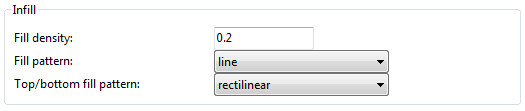
\includegraphics[keepaspectratio=true,width=1.0\textwidth]{expertmode/infill_pattern_settings.png}
\caption{Infill pattern settings.}
\label{fig:infill_pattern_settings}
\end{figure}

Slic3r offers several infill patterns, four regular, and three more exotic flavours.  The numbers given in brackets below each figure are a rough estimate of material used and time taken for a simple 20mm cube model\footnote{Taken from http://gcode.ws}.  Note that this is only indicative, as model complexity and other factors will affect time and material.

\begin{figure}[H]
\centering
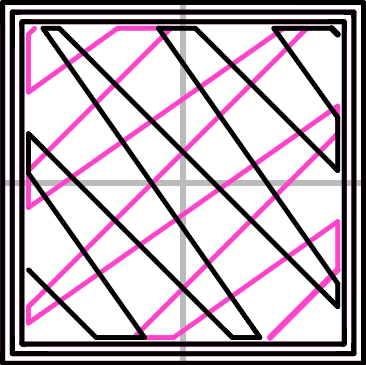
\includegraphics[keepaspectratio=true,width=0.2\textwidth]{expertmode/infill_line.png}
\caption{Infill pattern: Line (344.51mm / 5m:20s)}
\label{fig:infill_line}
\end{figure}

\begin{figure}[H]
\centering
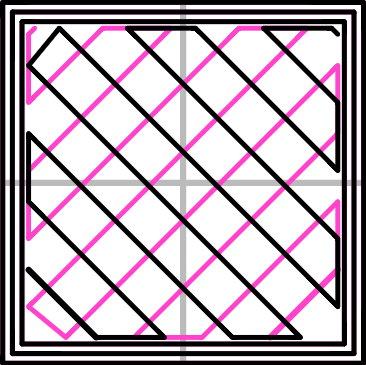
\includegraphics[keepaspectratio=true,width=0.2\textwidth]{expertmode/infill_rectilinear.png}
\caption{Infill pattern: Rectilinear (350.57mm / 5m:23s)}
\label{fig:infill_rectilinear}
\end{figure}

\begin{figure}[H]
\centering
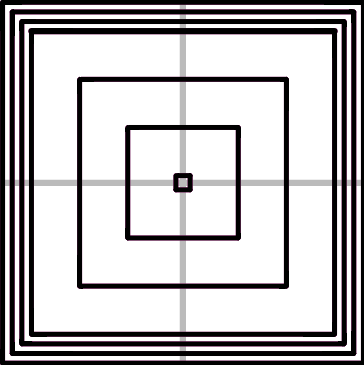
\includegraphics[keepaspectratio=true,width=0.2\textwidth]{expertmode/infill_concentric.png}
\caption{Infill pattern: Concentric (351.80mm / 5m:30s)}
\label{fig:infill_concentric}
\end{figure}

\begin{figure}[H]
\centering
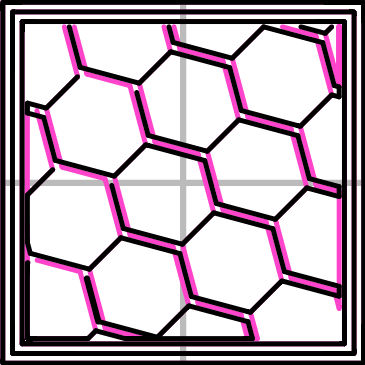
\includegraphics[keepaspectratio=true,width=0.2\textwidth]{expertmode/infill_honeycomb.png}
\caption{Infill pattern: Honeycomb (362.73mm / 5m:39s)}
\label{fig:infill_honeycomb}
\end{figure}

\begin{figure}[H]
\centering
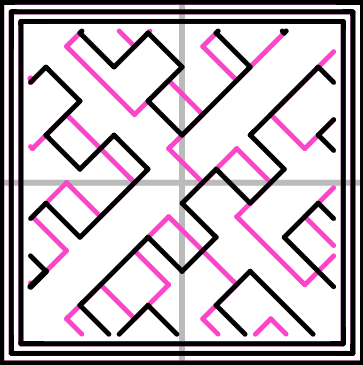
\includegraphics[keepaspectratio=true,width=0.2\textwidth]{expertmode/infill_hilbertcurve.png}
\caption{Infill pattern: Hilbert Curve (332.82mm / 5m:28s)}
\label{fig:infill_hilbertcurve}
\end{figure}

\begin{figure}[H]
\centering
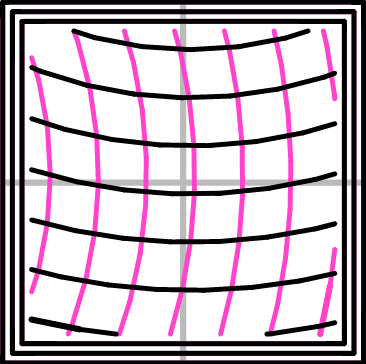
\includegraphics[keepaspectratio=true,width=0.2\textwidth]{expertmode/infill_archimedeanchords.png}
\caption{Infill pattern: Archimedean Chords (333.66mm / 5m:27s)}
\label{fig:infill_archimedeanchords}
\end{figure}

\begin{figure}[H]
\centering
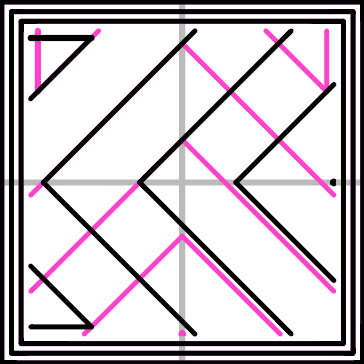
\includegraphics[keepaspectratio=true,width=0.2\textwidth]{expertmode/infill_octagramspiral.png}
\caption{Infill pattern: Octagram Spiral (318.63mm / 5m:15s)}
\label{fig:infill_octagramspiral}
\end{figure}


Certain model types are more suited for a particular pattern, for example organic versus mechanical types.  Figure \ref{fig:complex_object_infill_comparison} shows how a honeycomb fill may suit this mechanical part better because each hexagon bonds with the same underlying pattern each layer, forming a strong vertical structure.

\begin{figure}[H]
\centering
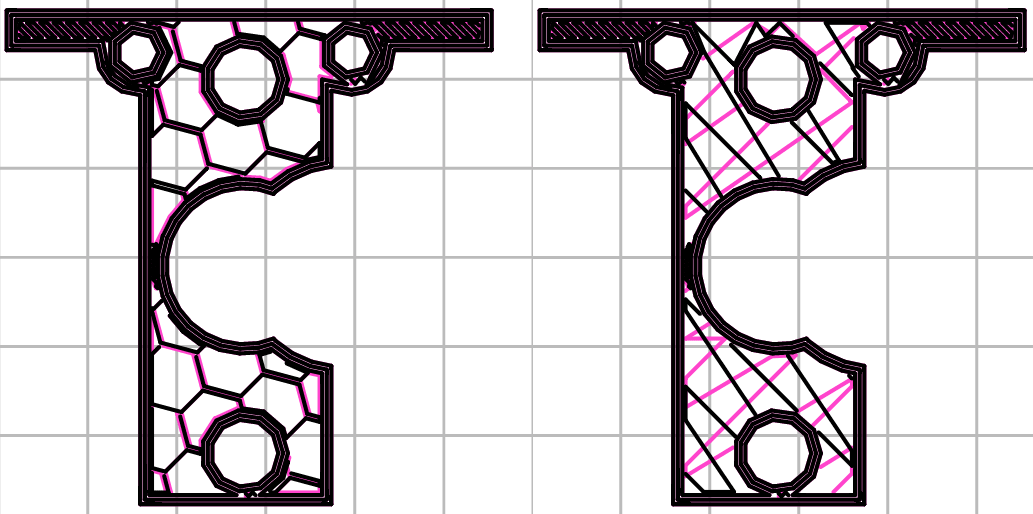
\includegraphics[keepaspectratio=true,width=0.75\textwidth]{expertmode/complex_object_infill_comparison.png}
\caption{Infill pattern comparison in a complex object. Left to Right: honeycomb, line}
\label{fig:complex_object_infill_comparison}
\end{figure}

Most models require only a low density infill, as providing more than, say, 50\% will produce a very tightly packed model which uses more material than required.  For this reason a common range of patterns is between 10\% and 30\%, however the requirements of the model will determine which density is best.  Figure \ref{fig:infill_pattern_densities} shows how the patterns change as the density increases.
\begin{figure}[H]
\centering
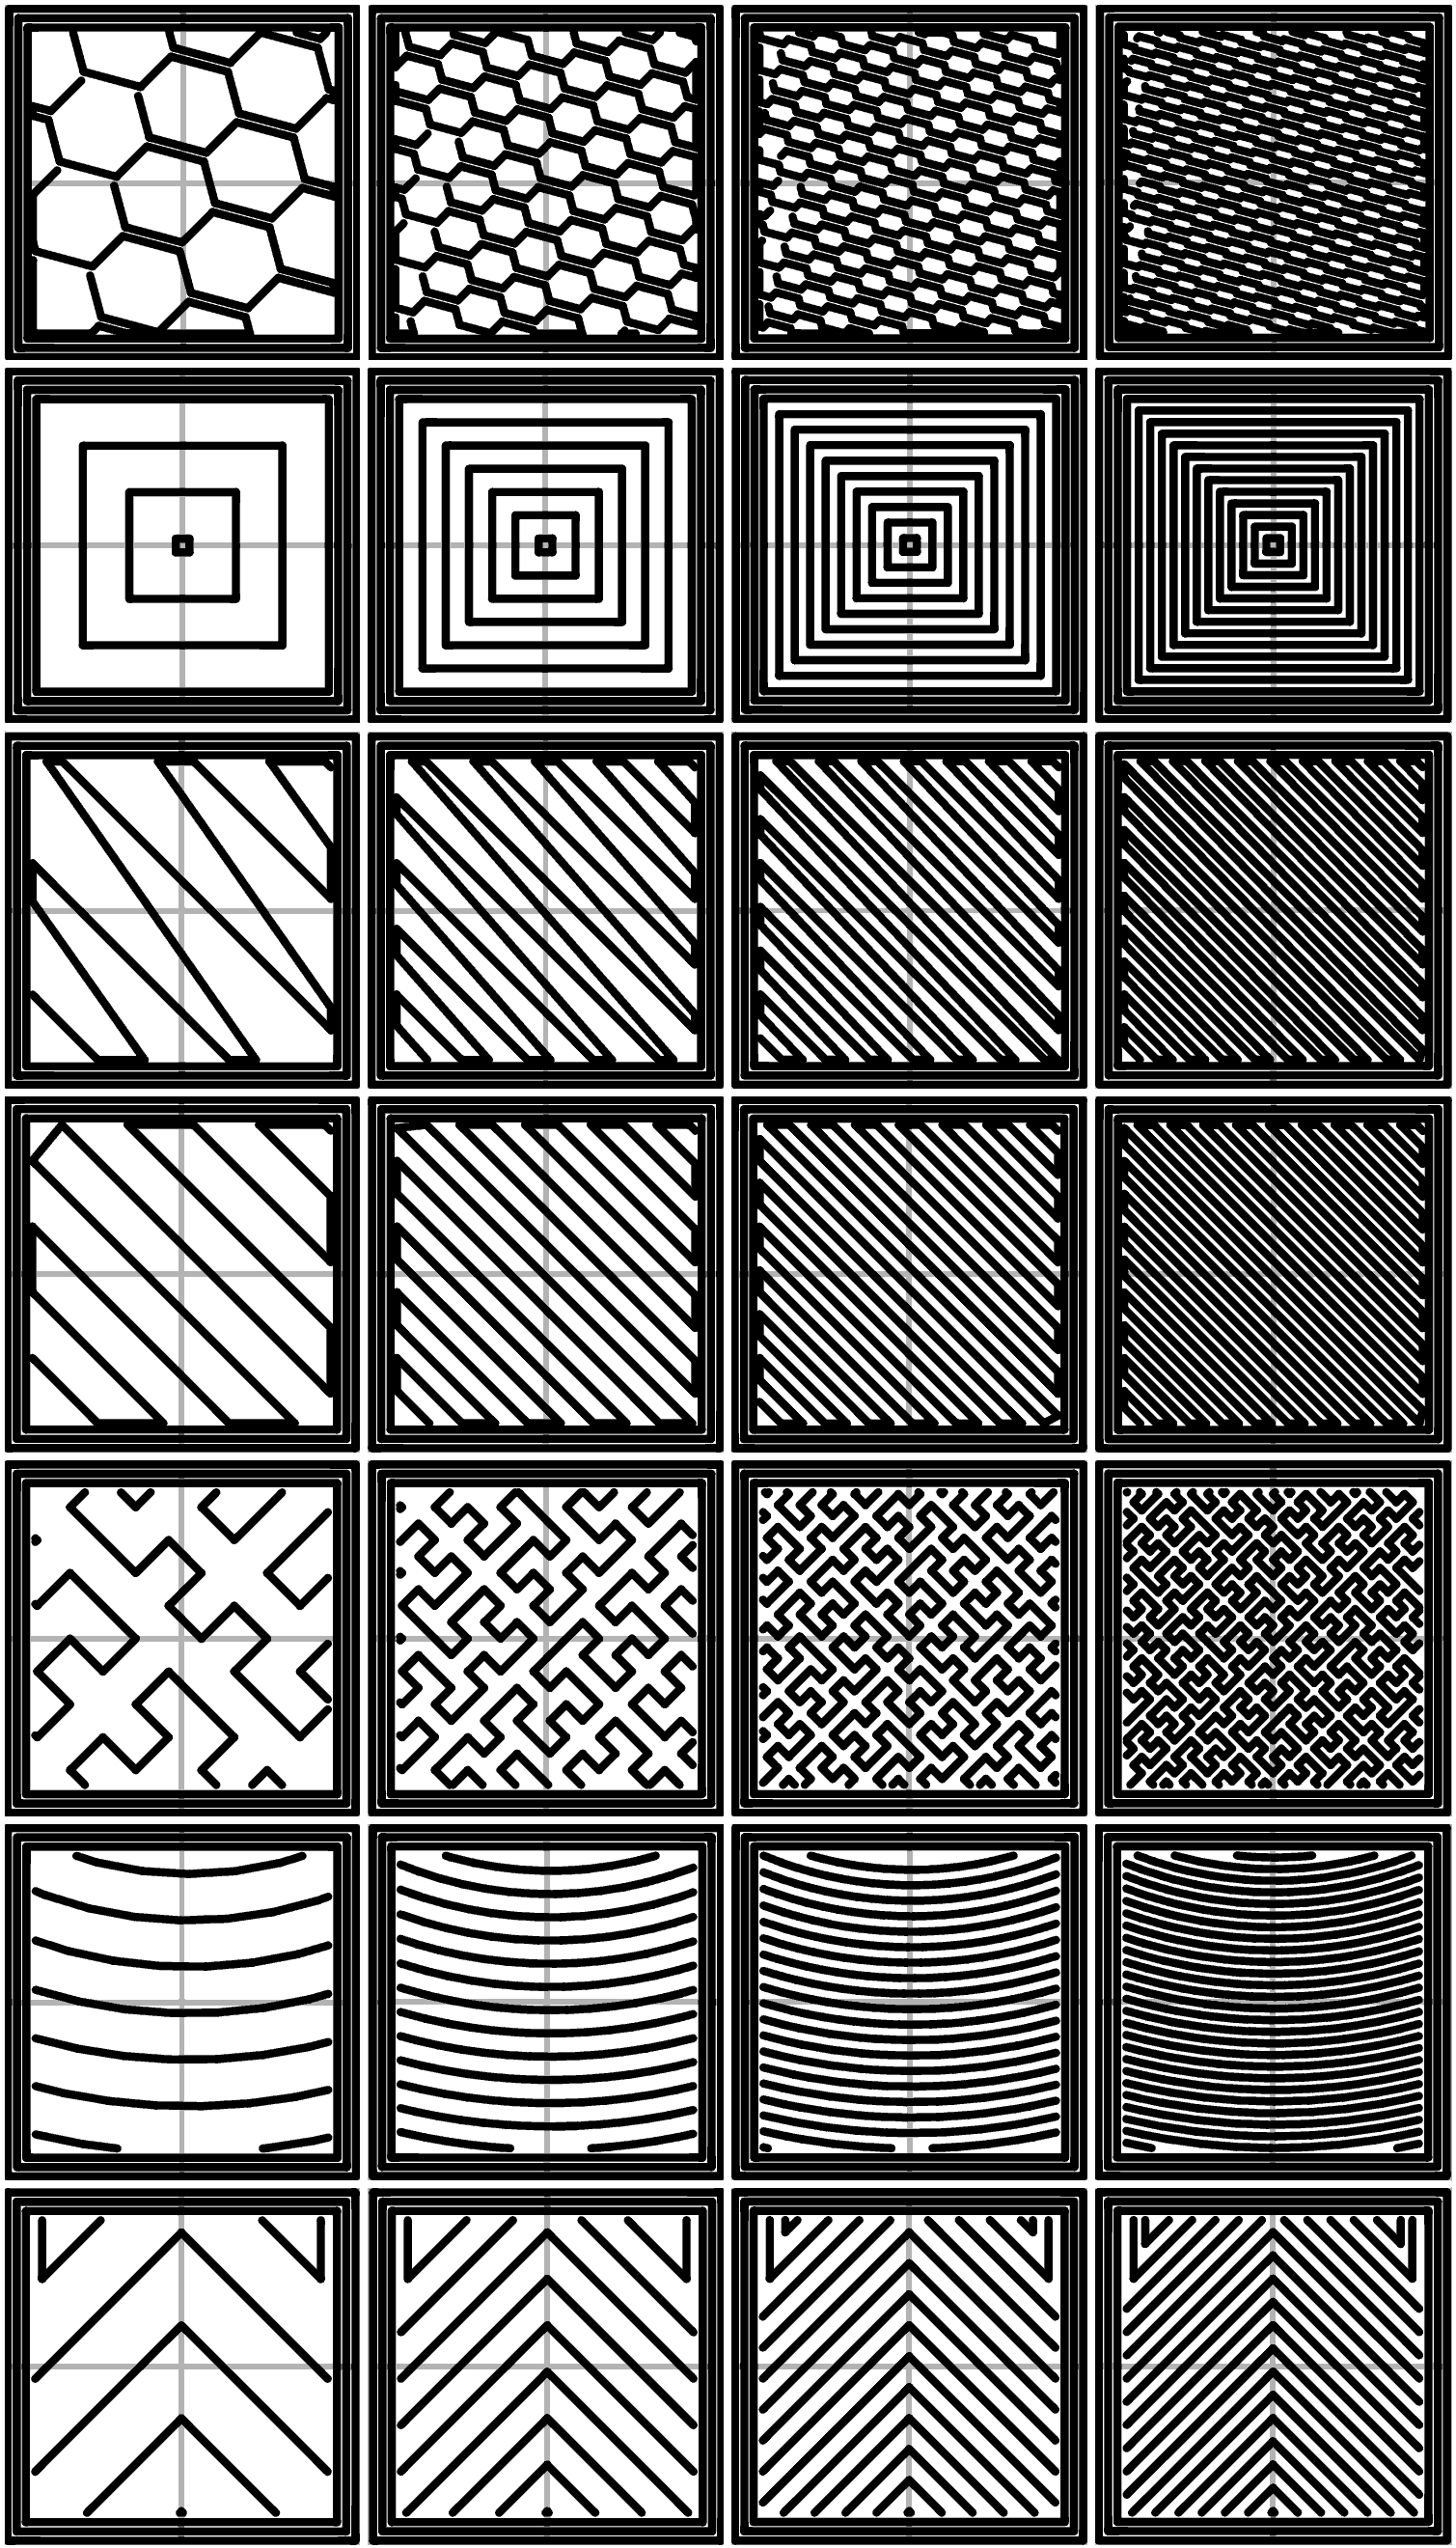
\includegraphics[keepaspectratio=true,width=0.7\textwidth]{expertmode/infills.png}
\caption{Infill patterns at varying densities. Left to Right: 20\%,40\%,60\%,80\%. Top to Bottom: Honeycomb, Concentric, Line, Rectilinear, Hilbert Curve, Archimedean Chords, Octagram Spiral}
\label{fig:infill_pattern_densities}
\end{figure}

% section infill_patterns_and_density (end)